\documentclass{article}
\usepackage[top=20mm, left=24mm, right=24mm]{geometry}
\usepackage{amsmath}
\usepackage{amsthm}
\usepackage{tikz}

\begin{document}
	\title{\textbf{Machine Learning - Ex. 6}}
	\author{Niv Shani - 311361661 {\quad} Anat Balzam - 205387954}
	\maketitle
	
	\subsection*{Question 1}
	$${H=\{h:X\rightarrow \{-1,+1\} , | x:h(x)=-1 | \leq 100\}}$$
	
	\renewcommand{\labelenumi}{\textbf{(\alph{enumi})}}
	\begin{enumerate}
		\item We can see that there is no constraint on the number of ${+1}$ that ${h}$ returns, and that ${h}$ can return ${-1}$ up to ${100}$ times. Thus, ${\forall Y = \{y_1, y_2, ..., y_{100}\} \in \{-1,+1\}^{100}}, \exists h\in H, s.t: \forall i: h(x_i) = y_i$.
		$${\Downarrow}$$
		$${VC(H) \geq 100}$$
		Let ${S \in X}$ be a subset of instances s.t ${|S|=101}$.\\
		We can look at the assignment ${Y=\{-1,-1,-1,...,-1\}}$. Since ${|x: h(x)=-1|\leq 100}$, there is no ${h \in H}$ s.t ${h(x_{101})=-1}$. Since there is a set of 100 points that is shattered by ${H}$, and no set of 101 points is:
		$${\textbf{VC(H) = 100}}$$
		
		\item We can use the same example from \textbf{(a)}, with the max number of ${-1}$ set to be 2019:
		$${H=\{h:X\rightarrow \{-1,+1\} , | x:h(x)=-1 | \leq 2019\}}$$
		Following the exact same proof, we have ${\textbf{VC(H) = 2019}}$.
		
		\item (1) Let ${X = \{(1,1), (-1,1), (0,0)\} \in \mathbf{R}^2}$. There are 8 possible assignments ${Y = \{y_1,y_2,y_3\}}$. We will show that for each assignment, there exists a hypothesis ${h \in H}$ s.t ${\forall (x_1,x_2) \in X,  h(x_1,x_2) = y_i}$.
		
		For each assignment ${Y =(y_1, y_2, y_3)}$ we can solve the system of linear equations:
		\begin{equation}
			\begin{pmatrix}
			  1 & 1 & 1\\
			  -1 & 1 & 1\\
			  0 & 0 & 1
			\end{pmatrix}
			\cdot
			\begin{pmatrix}
				w_1\\
				w_2\\
				b
			\end{pmatrix}
			= 
			\begin{pmatrix}
				y_1\\
				y_2\\
				y_3
			\end{pmatrix}
		\end{equation}
		Notice that:
		\begin{equation*}
			det
			\begin{pmatrix}
				1 & 1 & 1\\
				-1 & 1 & 1\\
				0 & 0 & 1
			\end{pmatrix} = 2 \geq 0
		\end{equation*}\\
		Therefore, the matrix is invertible, so there is always a solution to equation \textbf{(1)}. Thus there are ${(w_1, w_2, b)}$ that satisfy the assignment - meaning, ${H}$ shatters ${X}$ {\Rightarrow} ${VC(H) \geq 3}$.
		
		(2) We will prove the following \textbf{Lemma 1}:\\
		
		${\forall z, z' \in \mathbf{R}^2}$ if ${h(z) = h(z') = y}$ then it holds that ${\forall \alpha \in [0,1],\quad h((1-\alpha)z + \alpha z') = y}$.\\
		
		Let ${z = (x_1, x_2), z' = (y_1, y_2)}$ s.t ${h(z) = h(z') = y}$. ${h}$ is defined by ${w_1, w_2, b}$. Since ${h(z) = h(z')}$, the product of the inner-products of ${z, z'}$ with the hyper-plane is positive. Let ${z^* = ((1-\alpha)z + \alpha z')}$ for ${\alpha \in [0,1]}$.\\
		
		We know that the following holds:
		\begin{equation*}
			sign(w_1x_1 + w_2x_2 + b) = sign(w_1y_1 + w_2y_2 + b) = sign(y)
		\end{equation*}
		We will now look at the inner product ${(z^* \cdot w)+ b}$.\\\\
		${z^* = (1-\alpha)z + \alpha z' = ((1-\alpha)x_1 + \alpha y_1, (1-\alpha)x_2 + \alpha y_2)}$\\\\
		Thus:
		\begin{align*}
		(z^* \cdot w)+ b & = w_1[(1-\alpha)x_1 + \alpha y_1] + w_2[(1-\alpha)x_2 + \alpha y_2] + b\\
		& = (1-\alpha)w_1x_1 + \alpha w_1y_1 + (1-\alpha)w_2x_2 + \alpha w_2y_2 + b\\
		& = (1-\alpha)w_1x_1 + \alpha w_1y_1 + (1-\alpha)w_2x_2 + \alpha w_2y_2 + b \textbf{+ (1-\alpha)b + \alpha b -b}\\
		& = (1 - \alpha)[w_1x_1 + w_2x_2 + b] + \alpha [w_1y_1 + w_2y_2 + b] +b -b\\
		& = (\underbrace{1 - \alpha}_{positive})[\underbrace{w_1x_1 + w_2x_2 + b}_{= sign(y)}] + \underbrace{\alpha}_{positive} [\underbrace{w_1y_1 + w_2y_2 + b}_{= sign(y)}]\\
		\end{align*}
		$${\Downarrow}$$
		$${sign(z^* \cdot w) = sign(y)}$$
		Hence, ${z, z'}$ and ${z^*}$ are all on the same side of the linear seperator. Meaning:
		$${h(z^*) = y \qed}$$\\
		
		Using \textbf{Lemma 1} we can proof that ${VC(H) < 4}$ by constructing a counter-example in several cases. \\
		Let ${A = {z_1, z_2, z_3, z_4} \in \mathbf{R}^2}$:
		\begin{itemize}
			\item If the convex hull of A forms a \textbf{line}, the labeling ${+ - + -}$ going along the line for example, is impossible.
			
			\item If the convex hull of A forms a \textbf{triangle}, then the labeling with ${+}$ (the three points of the triangle) and ${-}$ (the interior point) is impossible.
			
			\item If the convex hull of A forms a \textbf{quadrilateral}, then following \textbf{Lemma 1} we proved above, setting ${z_1, z_2}$ to be the points separated by the long diagonal, it is impossible that ${z_3, z_4}$ are label differently.
		\end{itemize}
	Since some set of 3 points is shattered by ${H}$, and no set of 4 points is,
	$${\textbf{VC(H) = 3}}$$
	
	\newpage
	\item Let ${X = \mathbf{R}^d}$, then:
	$${H = \{h: \exists w \in \mathbf{R}^d , b \in \mathbf{R}\quad s.t\quad h(x) = \begin{cases}
		+1\quad w\cdot x > 0\\
		-1\quad w\cdot x \leq 0
		\end{cases}}\}$$
	
	Firstly, we can generalize the proof from \textbf{(c)} to construct the proof for dimension ${d}$ using an invertible matrix in the same way. From that we can conclude:
	$${VC(H) \geq d + 1}$$\\
	Secondly, Let ${X = \{x_1, x_2, ... , x_{d+2}\}}$ a set of ${d + 2}$ vectors in a ${d + 1}$-dimensional space. Therefore, ${X}$ is linearly dependent, meaning there exists ${x_j \in X}$ s.t:
	$${x_j = \sum_{i \not = j}^{d + 1} a_ix_i}\qquad \{a_1,...,a_{d+1} \in \mathbf{R}\}$$
	and not all ${a_i}$ are zeros.\\
	We take the assignment that sets ${y_j = -1}$, and ${y_i = sign(a_i)}$ (if ${a_i = 0}$, set ${y_i = 1}$).\\
	
	Notice that we define ${sign(y_i)}$ to be the label that ${h}$ has given the instance ${x_i}$. Therefore, it holds: ${y_i = sign(a_i) = sign(w\cdot x_i + b)}$.\\
	
	Looking at ${x_j}$, we get:
	$${sign(w\cdot x_j + b) = sign(\sum_{i \not = j}^{d + 1}a_i\cdot(w\cdot x_i +b)) > 0}$$
	But ${y_j = -1}$ as we declared above {\Rightarrow} contradiction.\\
	Hence there exists an assignment of ${d + 2}$ points not achievable by ${H}$. Meaning,
	${VC(H) < d + 2}$.
	$${\Downarrow}$$
	$${\textbf{VC(H) = d + 1}}$$	

	\end{enumerate}
	\newpage
	\subsection*{Question 2}
	We define the concept class ${C}$ to be to be all the conjuctions of at most ${n}$ Boolean literlas ${\{x_1,x_2,...,x_n\}}$, where a Boolean literal is either a variable ${x_i, i \in [1,n]}$ or it's negation, ${\overline{x_i}}$.\\
	
	\noindent
	Since each of the ${n}$ literals can be included positively, with negation, or not included at all - we have ${|C| = |H| = 3^n}$.\\
	
	\noindent
	\textbf{(*)} Let ${c \in C}$ be a conjunction of at most ${n}$ Boolean literals, and let ${b = \{b_1,...,b_k\}, \thickspace k \in [1,n]}$ be a positive assignment for ${c}$. Note:
	\begin{itemize}
		\item If ${b_i = 1}$, then for sure ${\overline{x_i} \not \in c}$, since ${\overline{1} = 0}$, making ${c = 0}$.
		\item If ${b_i = 0}$, then following the same rule, ${x_i \not \in c}$.
	\end{itemize}
	
	\subsubsection*{The Algorithm}
	\begin{enumerate}
		\item Start with the hypothesis ${h = x_1\land \overline{x_1}\land x_2 \land \overline{x_2}\land ... \land x_n \land \overline{x_n}}$.
		
		\item \textbf{For each positive training instance ${\overrightarrow{x}}$} (where ${c(\overrightarrow{x}) = true}$), follow \textbf{(*)} and rule out all relevant literals ${l_i \in \overrightarrow{x}}$ from ${h}$.
	\end{enumerate}

	\noindent
	We end up with ${h = l_{i_1} \land l_{i_2} \land ... \land l_{i_k}}$, which is also consistent with the negative instances, since no literal which causes ${h}$ to be \textbf{false} is in ${h}$.\\
	$${\Downarrow}$$
	\begin{center}
			${h(\overrightarrow{x}) = T}$ for positive training instances x.
	\end{center}
	
	\subsubsection*{Sample Complexity}
	Since every instance has ${n}$ attributes, we have ${|H| = 3^n}$.\\
	We want to ensure that the probability of ${h}$ to have error is less than ${\epsilon}$, is bounded by ${1 - \delta}$.\\
	Meaning: ${Prֿֿ\left[error_D(h) > \epsilon\right] < \delta}$.\\
	
	\noindent
	As seen in class, in order to reduce the failure probability below {$\delta$}, we need:
	\begin{align*}
		m & \geq \frac{1}{\epsilon}\ln{\frac{|H|}{\delta}}\\
		& = \frac{1}{\epsilon}\cdot \left(\ln{|H|} + \ln{\frac{1}{\delta}}\right)\\
		& = \frac{1}{\epsilon}\cdot \left(\cdot\ln{3^n} + \ln{\frac{1}{\delta}}\right) = \thickspace \frac{n}{\epsilon}\ln{3} + \frac{1}{\epsilon}\ln{\frac{1}{\delta}}
	\end{align*}
	$${\Downarrow}$$
	\begin{center}
		Meaning the sample complexity ${\textbf{m}}$ is polynomial in ${\frac{1}{\epsilon}, \frac{1}{\delta}}$ and ${n}$.
	\end{center}

	\subsubsection*{Time Complexity}
	Each step of the learning process algorithm is polynomial - checking one instance by considering ${O(n)}$ literals to obtain a consistent expression.\\
	
	\noindent
	Meaning the time complexity of the algorithm is polynomial in ${\frac{1}{\epsilon}, \frac{1}{\delta}}$ and ${n}$.\\

	\noindent
	\textbf{Hence, conjunctions of ${n}$ literals are PAC-Learnable.} \qedsymbol
	
	
	\newpage
	\subsection*{Question 3}
	
	Firstly, notice that given an isosceles triangle with its head vertex in ${(0,0)}$ and its sides parallel to the axes, we can define it using only the \textbf{median} to the base.\\
	
	\noindent
	Lets denote the median length to be ${d}$.\\
	Denote the median of the target triangle to be ${d^*}$.\\
	Each instance ${x \in \mathbf{R}^2}$ is drawn from an unknown distribution ${\mathcal{D}}$ and contains two features:
	\begin{itemize}
		\item the instance's position: ${(x_1,x_2)}$
		\item a target label: ${+1}$ if its inside the circle or ${-1}$ otherwise.
	\end{itemize}

	\noindent
	We can choose ${d}$ to be the hypothesis (median ${d}$ is well-defining a triangle, as explained above) that is fitting the tightest triangle around the positive instances, so that all of them lie inside it.\\
	
	\noindent
	Note that the error trapezoid is given in the area between the target triangle's base, and our hypothesis triangle's base - denote this area to be ${E_d}$.\\
	
	\begin{center}
		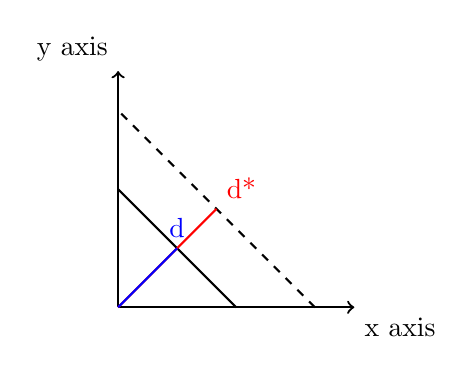
\begin{tikzpicture}
			\draw[thick, ->] (0,0) -- (3,0) node[anchor=north west] {x axis};
			\draw[thick, ->] (0,0) -- (0,3) node[anchor=south east] {y axis};
			\draw[thick, -] (1.5,0) -- (0,1.5);
			\draw[thick, dashed] (2.5,0) -- (0,2.5);
			\draw[thick, red] (0,0) -- (1.25,1.25) node [anchor=south west] {d*};
			\draw[thick, blue] (0,0) -- (0.75,0.75) node [anchor=south] {d};
		\end{tikzpicture}
	\end{center}
	
	\noindent
	We split the proof in two cases. Define:
	$${d^\epsilon = \underset{d}{\arg \min}\quad Pr\left[(x_1,x_2) \in E_d\right]}$$
	
	\subsubsection*{Case 1 (trivial)}
	If ${d^\epsilon \leq d}$ then ${E_{d^\epsilon} \leq E_d}$ - hence the probability of an instance being inside the error-area ${E_d}$ is less then ${\epsilon}$.
	
	\subsubsection*{Case 2}
	The probability of ${h}$ to be consistent with an instance ${x_i}$ where ${x_i \not \in E_d}$ is ${1 - \epsilon}$.\\
	Therefore, the probability of ${h}$ to be consistent with ${m}$ independent samples, is ${(1 - \epsilon)^m}$.\\
	As we saw in class, we can bound this probability, using sample size of ${m \geq \frac{\ln{\frac{1}{\delta}}}{\epsilon}}$:
	\begin{align*}
		(1 - \epsilon)^m & \leq \exp{(-\epsilon m)}\\
		& \leq \exp{(-\ln{\frac{1}{\delta}})}\\
		& = \exp{(\ln{\delta})}\\
		& = \textbf{\delta}
	\end{align*}
	$${\Downarrow}$$
	$${\text{the probability of \epsilon-bad h to be consistent is bounded by \delta}}$$\\
	\noindent
	Concluding, L will output, with probability of at least ${(1 - \delta)}$ an hypothesis ${h \in H}$ s.t ${error_D(h) \leq \epsilon}$, in time that is polynomial in ${\frac{1}{\epsilon}}$, ${\frac{1}{\delta}}$, ${n = 2}$ and ${|C| = |H|}$.\\
	
	\noindent
\textbf{Therefore, C is PAC-Learnable by L using H.}
	
	
	
	
	
	
	
	
	
	
	
	
	
	
	
	


\end{document}